\documentclass{article}
\usepackage{enumerate}
\usepackage{amsfonts, amscd, amsmath, amssymb}
\usepackage{graphicx}

\oddsidemargin -0.3cm
\evensidemargin 0cm
\textwidth 16.5cm
\textheight 21cm

\def\N{\mathbb N}
\def\Z{\mathbb Z}
\def\Q{\mathbb Q}
\def\R{\mathbb R}
\def\C{\mathbb C}

\title{Tema 3. Filtratge del Senyal}
\author{{\small J.L. Lisani (UIB)}}
\date{}

\begin{document}
\maketitle

\tableofcontents

\section{Introducci\'o}
Un {\bf filtre} o {\bf sistema} \'es qualsevol proc\'es que modifica un senyal, 
anomenat senyal d'entrada, per donar lloc a un nou senyal o senyal de sortida.

Esquem\`aticament els sistemes es representen amb diagrames de blocs:

\begin{figure}[htbp]
\begin{center}
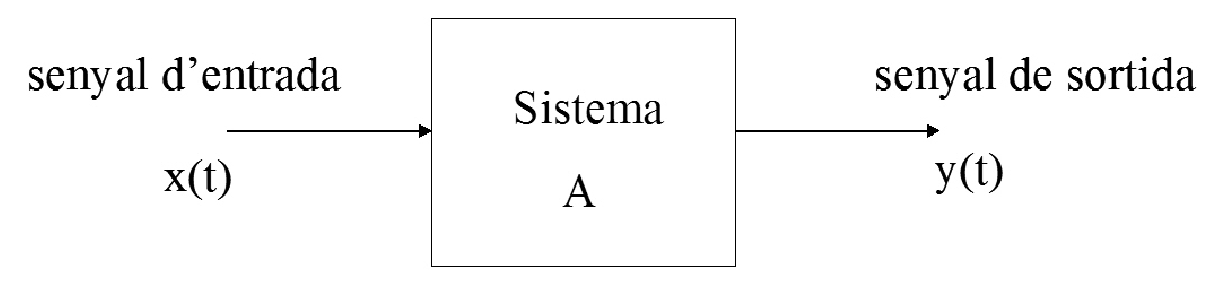
\includegraphics[width=9cm]{imatges/sistemaB.eps}
\caption{Representaci\'o esquem\`atica d'un sistema o filtre}
\label{sistema.fig}
\end{center}
\end{figure}

Matem\`aticament un filtre es modela com un operador entre dos espais de funcions:
\[
\begin{array}{crcl}
 A: & X & \longrightarrow & Y\\
    & x(t) & \longrightarrow & y(t)=A(x(t))
\end{array}
\]

\section{Propietats dels filtres}
Els filtres es classifiquen pel seu comportament respecte als senyals d'entrada.
Entre les propietats que poden tenir els filtres destaquen les seg\"uents:
\begin{itemize}
\item {\bf Linealitat}. Un filtre $A:X \rightarrow Y$ \'es lineal si
\newline
\newline
\begin{tabular}{ll}
i) $\forall u,v \in X$ & $A(u+v)=A(u)+A(v)$\\
ii)$\forall u \in X, \forall \lambda \in \C$ & $A(\lambda u)=\lambda A(u)$
\end{tabular}
\item {\bf Causalitat}. Un filtre $A:X \rightarrow Y$ \'es causal (o realitzable) si
\[
\forall t < t_0 \qquad x_1(t)=x_2(t) \Longrightarrow A(x_1(t))=A(x_2(t)) \qquad \forall t < t_0
\]
Aquesta propietat expressa la propietat f\'\i sica de que la resposta d'un sistema fins
a un temps $t_0$ no dep\`en m\'es que del passat anterior a $t_0$. En particular aix\'o
implica que la resposta del sistema no interv\'e en la entrada. La causalitat \'es una 
condici\'o necess\`aria perqu\`e el filtre sigui realitzable.
\item {\bf Invari\`ancia}. Un filtre $A:X \rightarrow Y$ \'es invariant o estacionari si
\[
\forall x \in X, \forall a \in \R \qquad A(x(t-a))=(Ax)(t-a)=y(t-a)
\]
Aquesta propietat implica que si l'entrada al sistema est\`a retardada un temps $a$, la sortida 
tamb\'e est\`a retardada el mateix temps $a$.
\end{itemize}

Les operacions cl\`assiques de tractament de senyal s'efectuen amb filtres causals, lineals i 
invariants.  
  
  
\section{Caracteritzaci\'o dels filtres lineals i invariants. Resposta impulsional}
Si un filtre $A$ \'es lineal i invariant \'es possible relacionar els senyals d'entrada
i sortida mitjan\c{c}ant una operaci\'o de convoluci\'o.

Sigui $x(t)$ el senyal d'entrada del filtre. En el tema anterior hem vist com qualsevol
funci\'o se pot escriure de la seg\"uent manera:
\[ 
x(t)=\int_{-\infty}^{+\infty} x(u) \delta(t-u) du 
\]
Per tant, per la linealitat del filtre, el senyal de sortida es pot calcular com
\[ 
y(t)=A(x(t))=\int_{-\infty}^{+\infty} x(u) A(\delta(t-u)) du =
\int_{-\infty}^{+\infty} x(u) (A\delta)(t-u) du 
\]
\noindent
on la darrera igualtat s'obt\'e per la invari\`ancia del filtre.

$A\delta$ representa la resposta del filtre a una delta de Dirac i s'anomena 
{\bf resposta impulsional del filtre}. La denotam com $h(t)=A\delta(t)$. 
Per tant 
\begin{equation}
\label{filtreconv}
y(t)=\int_{-\infty}^{+\infty} x(u) h(t-u) du=x(t) * h(t)
\end{equation}
 
\noindent
{\bf Propietat}. Si $A$ \'es causal llavors $h(t)=0, \forall t < 0$.

\noindent
{\it Dem}. Podem descomposar la integral (\ref{filtreconv}) en dues parts:
\[
y(t)=\int_{-\infty}^{+\infty} x(u) h(t-u) du=\int_{-\infty}^{t} x(u) h(t-u) du + 
\int_{t}^{+\infty} x(u) h(t-u) du
\]
Si el filtre \'es causal la seva sortida a l'instant $t$ no pot dependre dels valors de $x(u)$ si
$u > t$, per tant la segona de les integrals en la suma anterior ha d'\'esser nul.la per a qualsevol
$x(u)$, $u \geq t$. En conseq\"u\`encia $h(t-u)=0$ si $u > t$, o equivalentment, $h(s)=0$ si $s < 0$.
\begin{flushright}
$\square$
\end{flushright}

\noindent
{\bf Definici\'o i Propietat}. Es diu que un filtre \'es {\bf estable} si la seva sortida est\`a
afitada quan l'entrada ho est\`a.

Podem afitar la sortida d'un filtre de la seg\"uent manera:
\[
\begin{array}{rcl}
|y(t)|=|(Ax)(t)| & = & 
|\int_{-\infty}^{+\infty} x(u) h(t-u) du| \leq \int_{-\infty}^{+\infty} |x(u)| |h(t-u)| du \leq \\
\\
                 & \leq & \sup_{u \in \R} |x(u)| \int_{-\infty}^{+\infty} |h(u)| du
\end{array}
\]

En conseq\"u\`encia, l'estabilitat es verificar\`a nom\'es si $\int_{-infty}^{+\infty} |h(u)| du < +\infty$,
\'es a dir, el filtre ser\`a estable nom\'es si $h(t)$ \'es integrable.


\section{Funcions de transfer\`encia}
Donat un filtre $A: X \rightarrow Y$ lineal i invariant, consideram la seva resposta davant una 
exponencial complexe: $x(t)=e^{i 2 \pi \xi t}$.
\[
\begin{array}{rcl}
y(t)=A(x(t)) & = & x(t)*h(t)=\int_{-\infty}^{+\infty} x(u) h(t-u) du = \int_{-\infty}^{+\infty} h(u) x(t-u) du =\\
\\
             & = & \int_{-\infty}^{+\infty} h(u) e^{i 2 \pi \xi (t-u)} du = 
                   e^{i 2 \pi \xi t} \int_{-\infty}^{+\infty} h(u) e^{-i 2 \pi \xi u} du =\\
\\
             & = & e^{i 2 \pi \xi t} \hat{h}(\xi)
\end{array}
\]

Aquest resultat implica que $e^{i 2 \pi \xi t}$ \'es un vector propi de $A$ i que $\hat{h}(\xi)$ 
(la transformada de Fourier de $h$ a la freq\"u\`encia $\xi$) \'es el seu valor propi associat.
$\hat{h}(\xi)$ s'anomena {\bf funci\'o de transfer\`encia} del filtre.

\vskip 0.3 cm
Per la linealitat de $A$, si podem descomposar $x(t)$ en una suma d'exponencials complexes 
(per exemple, mitjan\c{c}ant la transformada inversa de Fourier), podrem escriure:
\[
x(t)=\int_{-\infty}^{+\infty} \hat{x}(\xi) e^{i 2 \pi \xi t} d\xi
\]
\[
y(t)=A(x(t)) = \int_{-\infty}^{+\infty} \hat{x}(\xi) A(e^{i 2 \pi \xi t}) d\xi = 
\int_{-\infty}^{+\infty} \hat{x}(\xi) \hat{h}(\xi) e^{i 2 \pi \xi t} d\xi
\]
La darrera integral \'es l'antitransformada de Fourier del producte de $\hat{x}(\xi)$ per
$\hat{h}(\xi)$. Com que $y(t)=x(t)*h(t)$, l'anterior equaci\'o expressa la coneguda propietat
$\widehat{x*h}=\hat{x}\hat{h}$.

\section{Classificaci\'o freq\"uencial dels filtres}
Recordem del tema 2 que la transformada de Fourier de la delta de dirac \'es igual a $1$, un 
valor constant per a totes les freq\"u\`encies. Aix\'o siginifica que la delta de Dirac
\'es un senyal que t\'e components espectrals en totes les freq\"u\`encies.

Per tant $h(t)$, com a resposta d'un sistema a una delta de Dirac, representa la resposta
del sistema a totes les freq\"u\`encies possibles i $\hat{h}(\xi)$ $\forall \xi$ representa tots 
els valors propis possibles del filtre. 

En funci\'o de la distribuci\'o d'aquests valors propis (\'es a dir, en funci\'o de $\hat{h}(\xi)$),
els filtres es classifiquen en:
\begin{itemize}
\item {\bf Filtres passa-baix}. S\'on aquells per als quals la funci\'o de transfer\`encia 
s'anul.la a partir d'una determinada freq\"u\`encia $\xi_T$ anomenada freq\"u\`encia de
tall ($\hat(\xi)=0$ $\forall |\xi| > \xi_T$). El filtre passa-baix ideal es modelitza com
una funci\'o indicatriu en freq\"u\`encia: $\hat{h}(\xi)={\cal X}_{[\xi_T, \xi_T]}$. No obstant,
l'antitransformada de Fourier d'aquesta funci\'o t\'e un suport infinit i \'es per tant
irrealitzable. En la pr\`actica, els filtres passa-baix mostren una decaiguda r\`apida dels valors
de $\hat{h}(\xi)$ a partir d'una certa freq\"u\`encia que \'es la que se considera freq\"u\`encia
de tall del filtre (veure la Figura \ref{figpassabaix}). Aquests filtres tenen la propietat 
d'eliminar les altes freq\"u\`encies dels senyals d'entrada.

\begin{figure}[htbp]
\begin{center}
\begin{tabular}{cc}
\includegraphics[width=3cm]{imatges/passabaixideal.eps} &
\includegraphics[width=3cm]{imatges/passabaixreal.eps}
\end{tabular}
\caption{Filtre passa-baix ideal i real (m\`odul de la funci\'o de transfer\`encia del filtre).}
\label{figpassabaix}
\end{center}
\end{figure}

\item {\bf Filtres passa-alt}. La funci\'o de transfer\`encia d'aquests filtres val zero per
davall de la freq\"u\`encia de tall ($\hat{h}(\xi)=0$ $\forall |\xi| < \xi_T$). Igual que 
en el cas dels filtres passa-baix, els filtres passa-alt ideals s\'on irrealitzables
(veure la Figura \ref{figpassaalt}). Aquests filtres eliminen les baixes freq\"u\`encies
dels senyals s'entrada.

\begin{figure}[htbp]
\begin{center}
\begin{tabular}{cc}
\includegraphics[width=3cm]{imatges/passaaltideal.eps} &
\includegraphics[width=3cm]{imatges/passaaltreal.eps}
\end{tabular}
\caption{Filtre passa-alt ideal i real (m\`odul de la funci\'o de transfer\`encia del filtre).}
\label{figpassaalt}
\end{center}
\end{figure}


\item {\bf Filtres passa-banda}. En aquest cas la funci\'o de transfer\`encia s'anul.la 
en un cert rang de freq\"u\`encies (Figura \ref{figpassabanda}). S'utilitzen per filtrar
determinades components freq\"uencials del senyals d'entrada.

\begin{figure}[htbp]
\begin{center}
\begin{tabular}{cc}
\includegraphics[width=3cm]{imatges/passabandaideal.eps} &
\includegraphics[width=3cm]{imatges/passabandareal.eps}
\end{tabular}

\caption{Filtre passa-banda ideal i real (m\`odul de la funci\'o de transfer\`encia del filtre).}
\label{figpassabanda}
\end{center}
\end{figure}

\end{itemize}

\subsection{Filtres anti-aliasing}
Un cas particular de filtres passa-baix s\'on els filtres anti-aliasing.
Recordem que l'aliasing es produeix quan l'espectre d'un senyal cont\'e  
valors no nuls en freq\"u\`encies fora de l'interval $[-\frac{1}{2T},+\frac{1}{2T}]$, 
on $T$ \'es el per\'\i ode de mostreig del senyal (secci\'o 2.3.3 del Tema 2).


Una manera d'evitar l'aliasing \'es filtrar, abans del mostreig, el senyal original
amb un filtre passa-baix amb freq\"u\`encia de tall $\xi_T=\frac{1}{2T}$. Aquest
filtre s'anomena filtre anti-aliasing.
 
Cal observar que l'aplicaci\'o del filtre anti-aliasing pot tenir com a efecte 
no desitjat l'aparici\'o del fen\`omen de Gibbs, motivat pel fet de reconstruir 
un senyal a partir d'una versi\'o truncada del seu espectre (Figura \ref{figgibbs}).

La figura seg\"uent ilustra l'efecte d'un filtre anti-aliasing en el sub-mostreig 
d'una imatge.

\begin{figure}[htbp]
\begin{center}
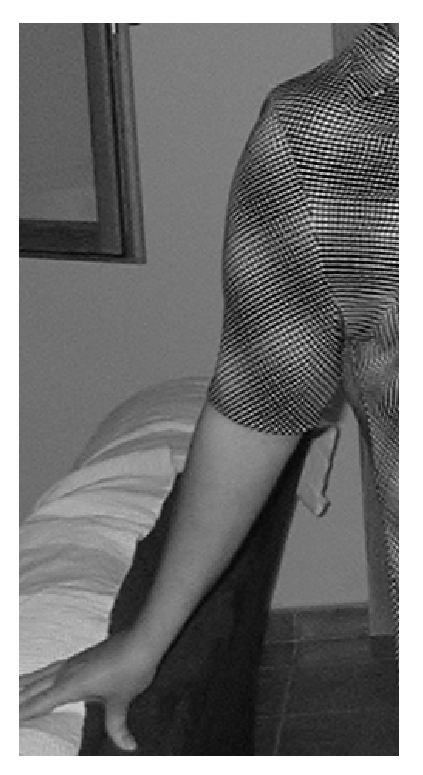
\includegraphics[width=8cm]{imatges/camisa.eps}\\
\begin{tabular}{cc}
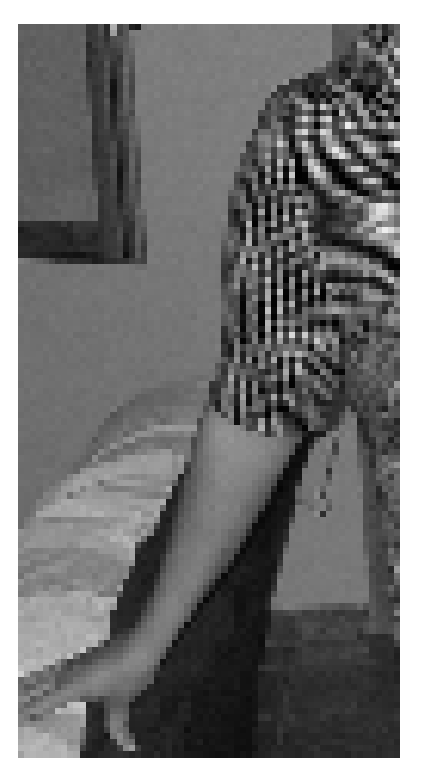
\includegraphics[width=2cm]{imatges/camisaIZ4.eps} &
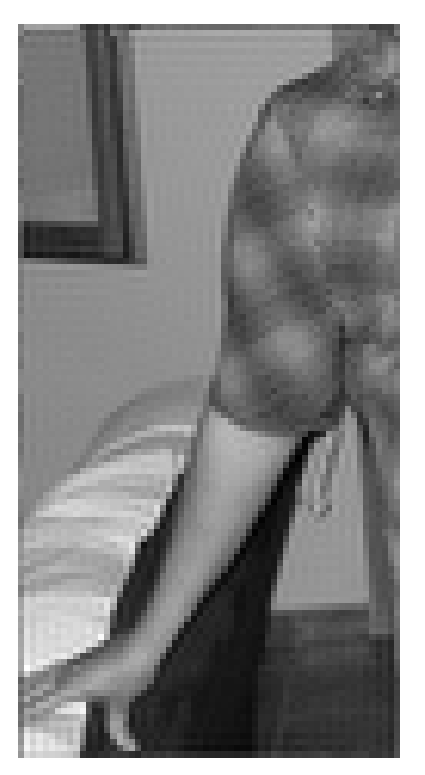
\includegraphics[width=2cm]{imatges/camisaFIZ4.eps}
\end{tabular}
\caption{Imatge original (a dalt) i dues versions sub-mostrejades (a baix) 
(s'ha pr\'es un pixel de cada quatre). El sub-mostreig equival a utilitzar un per\'iode 
de mostreig 4 vegades superior a l'original. La conseq\"u\`encia \'es l'aliasing
que es pot observar en la imatge de inferior esquerra. L'aplicaci\'o d'un filtre
anti-aliasing evita aquest fen\`omen (imatge inferior dreta).}
\label{figaliasing}
\end{center}
\end{figure}

\begin{figure}[htbp]
\begin{center}
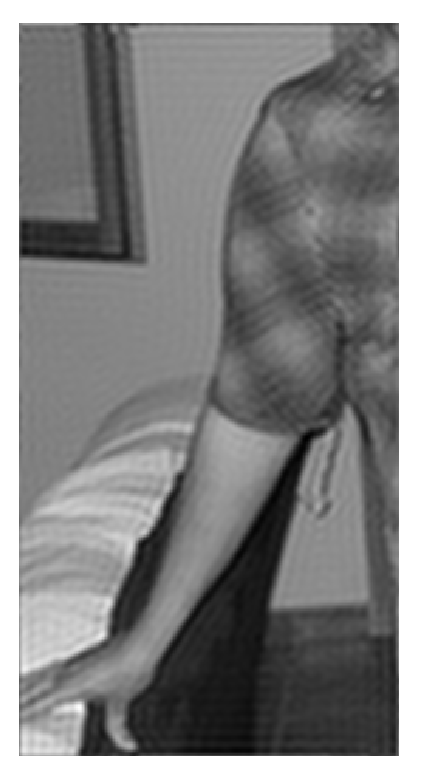
\includegraphics[width=8cm]{imatges/camisaF.eps}
\caption{Resultat d'aplicar el filtre anti-aliasing a la imatge original 
de la Figura anterior. Observar l'efecte de Gibbs. El sub-mostreig d'aquesta 
imatge ens d\'ona la imatge inferior dreta de la Figura anterior.}
\label{figgibbs}
\end{center}
\end{figure}
 
 
\section{Filtres discrets}
Els filtres discrets es defineixen i classifiquen de manera an\`aloga als 
continus o anal\`ogics. Si denotam per $X_D$ i $Y_D$ dos espais de funcions discretes,
un filtre discret $A$ \'es un operador entre ambd\'os espais.
En particular, el filtre discret $A:X_D \rightarrow Y_D$
\'es lineal i invariant si
\begin{enumerate}[i)]
\item $A(\lambda_1 x_1[n] + \lambda_2 x_2[n])=\lambda_1 A(x_1[n]) + \lambda_2 A(x_2[n])$
\item $A(x[n-n_0])=(Ax)[n-n0]$
\end{enumerate}
De la mateixa manera que per senyals continus podiem escriure un senyal $x(t)$ com
$x(t)=\int_{-\infty}^{+\infty} x(u) \delta(t-u) du$, per senyals discrets poder dir
que
\[
x[n]=\sum_{m=-\infty}^{+\infty} x[m] \delta[n-m]
\]
\noindent
on $\delta[n]=\begin{cases} 1 & \mathrm{si} \quad n=0\\ 0 & \mathrm{altrament}
\end{cases} \quad$ \'es la {\bf delta de Dirac discreta}.

Si el filtre $A$ \'es lineal i invariant llavors
$
A(x[n])=\sum_{m=-\infty}^{+\infty} x[m] (A\delta)[n-m]
$.
Si definim $h[n]=(A\delta)[n]$, llavors 
\begin{equation}
\label{filtreDconv}
y[n]=A(x[n])=\sum_{m=-\infty}^{+\infty} x[m] h[n-m]
\end{equation}
\noindent
aquesta darrera expressi\'o defineix la {\bf convoluci\'o discreta} de $x[n]$ i $h[n]$,
i es denota $x[n]*h[n]$. $h[n]$ rep el nom de {\bf resposta impulsional} del filtre discret.

\vskip 0.2 cm

Si $h[n]$ t\'e suport finit la suma (\ref{filtreDconv}) es realitzar\`a en un nombre
finit d'iteracions. Els  filtres amb $h[n]$ amb suport finit reben el nom de {\bf filtres 
amb resposta impulsional finita} o filtres {\bf FIR}.

\vskip 0.2 cm
\noindent
{\bf Definici\'o i Propietat}. Un filtre discret \'es causal si $A(x[n])$ no dep\`en dels 
valors de $x[m]$ quan $m > n$. Un filtre discret lineal i invariant \'es causal si i
nom\'es si $h[n]=0$ quan $n < 0$.

\noindent
{\it Dem}. La demostraci\'o \'es an\`aloga a la de la propietat equivalent per a filtres
continus.

\subsection{Funci\'o de transfer\`encia}
Al igual que per als filtres anal\`ogics, en el cas dels filtres discrets lineal i 
in\-va\-riants es cumpleix:
\[
\begin{array}{rcl}
A(e^{i 2 \pi \xi n}) & = & e^{i 2 \pi \xi n} * h[n] = 
                           \sum_{k=-\infty}^{+\infty} e^{i 2 \pi \xi m} h[n-m] =\\ \\
                     & = & \sum_{k=-\infty}^{+\infty} e^{i 2 \pi \xi (n-k)} h[k] =
                           e^{i 2 \pi \xi n} \sum_{k=-\infty}^{+\infty} h[k] e^{-i 2 \pi \xi k} 
\end{array}
\]
per tant $e^{i 2 \pi \xi n}$ \'es un vector propi del filtre i 
\[ 
h_T(\xi)=\sum_{k=-\infty}^{+\infty} h[k] e^{-i 2 \pi \xi k}
\]
\noindent
\'es el valor propi corresponent.
$h_T(\xi)$ \'es la {\bf funci\'o de transfer\`encia del filtre discret}. Cal observar
que aquesta \'es una funci\'o cont\'\i nua.

\vskip 0.3 cm
Consideram ara l'efecte d'aplicar un filtre discret FIR amb $N$ mostres 
damunt un senyal finit $x[n]$ format per $N$ mostres.


\subsection{Convoluci\'o circular}
En una situaci\'o pr\`actica es treballa amb senyals mostrejats amb un nombre finit 
($N$) de mostres. Donats dos senyals discrets finits $x[n]$ i $y[n]$ formats 
per $N$ mostres i perioditzats, definim la {\bf convoluci\'o circular} de $x$ i $y$
com:
\begin{equation}
\begin{array}{rcl}
(x \circledast y)[n] & = & x[n] \circledast y[n]=\sum_{m=0}^{N-1} x[m] y[n-m]=\\\\
 & = & \sum_{m=0}^{N-1} x[n-m]y[m] \qquad \qquad \qquad  n=0, \cdots,N-1
\end{array}
\end{equation}
 
Per la periodicitat de $x$ i $y$, $(x \circledast y)$ \'es tamb\'e peri\`odica de 
per\'\i ode $N$ i l'equaci\'o anterior defineix els seus valors en un per\'\i ode.
 
\vskip 0.2 cm
\noindent
{\bf Propietat \ref{convcircP1} \label{convcircP1}}. 
$x[n] \circledast y[n] = IDFT ( \hat{x}[k] \hat{y}[k] )$.

\noindent
{\it Dem}. Consideram primer la convoluci\'o d'un senyal $y[n]$ amb 
$N$ mostres d'una exponencial complexa:
\[
\begin{array}{rcl}
y[n] \circledast e^{i 2 \pi \frac{k}{N} n} & = & e^{i 2 \pi \frac{k}{N} n} \circ y[n] =
\sum_{m=0}^{N-1} y[m] e^{i 2 \pi \frac{k}{N} (n-m)} =\\\\
 & = & e^{i 2 \pi \frac{k}{N} n} \sum_{m=0}^{N-1} y[m] e^{-i 2 \pi \frac{k}{N} m}=\\\\
 & = & e^{i 2 \pi \frac{k}{N} n} \hat{y}[k]
\end{array}
\]
\noindent 
La f\`ormula de la IDFT del senyal $\hat{x}[k]$ ens permet expressar $x[n]$ com una
suma de exponencials, de manera que
\[
\begin{array}{rcl}
x[n] \circledast y[n] & = & 
(\frac{1}{N} \sum_{k=0}^{N-1} \hat{x}[k] e^{i 2 \pi \frac{k}{N} n}) \circledast y[n] =\\\\
 & = & \sum_{k=0}^{N-1} \hat{x}[k] (e^{i 2 \pi \frac{k}{N} n} \circledast y[n]) =
 \frac{1}{N} \sum_{k=0}^{N-1} \hat{x}[k] \hat{y}[k] e^{i 2 \pi \frac{k}{N} n} 
\end{array}
\]
\noindent 
i aquesta darrera expressi\'o \'es la IDFT del producte de $\hat{x}[k]$ per $\hat{y}[k]$.
\begin{flushright}
$\square$
\end{flushright}

\vskip 0.3 cm
\noindent
{\bf Propietat \ref{convcircP2} \label{convcircP2}}. {\bf Relaci\'o entre la convoluci\'o 
convencional i la convoluci\'o circular}.
Siguin $x[n]$ i $y[n]$ dos senyals discrets finits amb $N$ i $M$ mostres respectivament.
Consideram els nous senyals $x'[n]$ i $y'[n]$, peri\`odics, de per\'iode $N+M-1$, definits,
en el seu per\'iode principal, afegint zeros a les mostres de $x[n]$ i $y[n]$:
\[
x'[n]=\begin{cases} x[n] & \mathrm{si} \qquad n=0,\cdots,N-1\\
0 & \mathrm{si} \qquad n=N, \cdots, N+M-1 \end{cases}
\]
\[
y'[n]=\begin{cases} y[n] & \mathrm{si} \qquad n=0,\cdots,M-1\\
0 & \mathrm{si} \qquad n=N, \cdots, N+M-1 \end{cases}
\]
\noindent
Llavors 
\[
x[n]*y[n]=\begin{cases} x'[n]\circledast y'[n] & \mathrm{si} \qquad n=0,\cdots,N+M-1\\
0 & \mathrm{altrament} \end{cases}
\]

\vskip 0.3 cm
\noindent
{\bf Propietat \ref{convcircP3} \label{convcircP3}}. 
{\bf Relaci\'o entre la sortida d'un filtre discret FIR i la DFT}.
La combinaci\'o de les dues propietats anteriors ens permet trobar una relaci\'o entre
la sortida d'un filtre discret FIR amb $M$ mostres amb la DFT de la seva resposta
impulsional i de la del senyal d'entrada.

L'equaci\'o (\ref{filtreDconv}) ens defineix la sortida d'un filtre amb resposta impulsional
$h[n]$ com $y[n]=x[n]*h[n]$. Si $h[n]$ est\'a format per $M$ mostres i $x[n]$ per $N$ mostres
el senyals de sortida estar\'a format per $N+M-1$ mostres i, per la propietat \ref{convcircP2}:
\[
y[n]=x'[n]\circledast h'[n]
\]
\noindent 
on $x'[n]$ i $y'[n]$ s\'on les funcions definides m\'es amunt.
Si ara aplicam la propietat \ref{convcircP1}:
\begin{equation}
y[n]=IDFT \{ \widehat{x'}[k] \widehat{h'}[k] \} \qquad \qquad n=0, \cdots, N+M-1
\end{equation}
\noindent 
on $\widehat{x'}[k]$ i $\widehat{h'}[k]$ s\'on les DFT de $x'[n]$ i $h'[n]$ respectivament.

\vskip 0.2 cm
A m\'es, podem interpretar $\widehat{h'}[k]$ com una versi\'o discretitzada de la funci\'o de 
transfer\`encia del filtre FIR: $\widehat{h'}[k]=h_T(\frac{k}{N+M-1})$.

\end{document} 